\startSolutions{isometry}{Affine Transformations}

\begin{enumerate}[!HW!, start=1]
\begin{multicols}{3}
\itemspade $\cos^{-1}\left(\dfrac{2}{\sqrt{2}\sqrt{10}}\right)\approx 63.4^\circ$
\itemspade $\cos^{-1}\left(\dfrac{-8}{\sqrt{10}\sqrt{14}}\right)\approx 132.5^\circ$

\itemspade $\cos^{-1}\left(\dfrac{3}{\sqrt{30}}\right)\approx 56.8^\circ$
\end{multicols}
\begin{multicols}{4}
\itemspade rigid motion
\itemspade rigid motion
\itemspade not a rigid motion
\itemspade not a rigid motion
\end{multicols}
\begin{multicols}{4}
\itemspade rigid motion
\itemspade rigid motion
\itemspade not a rigid motion
\itemspade rigid motion
\end{multicols}

\begin{multicols}{2}
\itemspade \mbox{}\\
\begin{tikzpicture}[scale=0.8]
\draw[help lines,dashed] (-3,-3) grid (3,3);
\gridlines{-3}{3}{-3}{3};
\draw[ultra thick, blue, -latex, shift={(2,2)}] (0,0) -- (1,0) node[above, midway] {$\bb v$};
\fill[cyan] (2,1) circle (0.15) node[left, xshift=-3] {$P$};
\fill[magenta] (3,1) circle (0.15) node[right, xshift=3] {$P'$};
\end{tikzpicture}

\itemspade \mbox{}\\
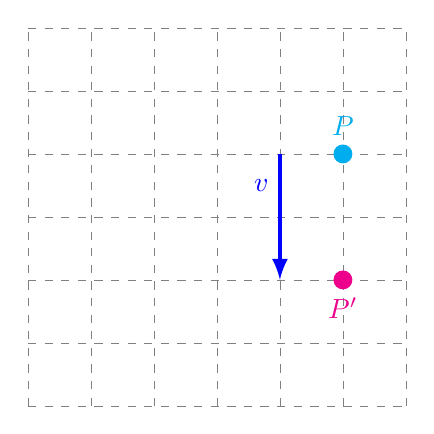
\begin{tikzpicture}[scale=0.8]
\draw[help lines,dashed] (-3,-3) grid (3,3);
\gridlines{-3}{3}{-3}{3};
\draw[ultra thick, blue, -latex, shift={(1,1)}] (0,0) -- (0,-2)  node[left, near start] {$\bb v$};
\fill[cyan] (2,1) circle (0.15) node[above, yshift=3] {$P$};
\fill[magenta] (2,-1) circle (0.15) node[below, yshift=-3] {$P'$};
\end{tikzpicture}
\end{multicols}

\begin{multicols}{2}
\itemspade \mbox{}\\
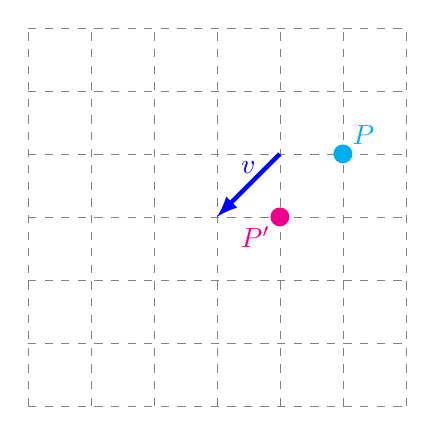
\begin{tikzpicture}[scale=0.8]
\draw[help lines,dashed] (-3,-3) grid (3,3);
\gridlines{-3}{3}{-3}{3};
\draw[ultra thick, blue, -latex, shift={(1,1)}] (0,0) -- (-1,-1)  node[above, midway] {$\bb v$};
\fill[cyan] (2,1) circle (0.15) node[above right] {$P$};
\fill[magenta] (1,0) circle (0.15) node[below left] {$P'$};
\end{tikzpicture}

\itemspade \mbox{}\\
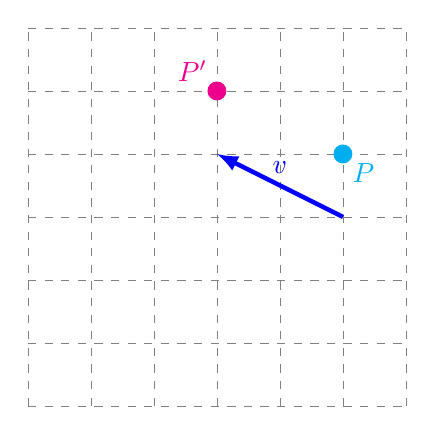
\begin{tikzpicture}[scale=0.8]
\draw[help lines,dashed] (-3,-3) grid (3,3);
\gridlines{-3}{3}{-3}{3};
\draw[ultra thick, blue, -latex, shift={(2,0)}] (0,0) -- (-2,1)  node[above, midway] {$\bb v$};
\fill[cyan] (2,1) circle (0.15) node[below right] {$P$};
\fill[magenta] (0,2) circle (0.15) node[above left] {$P'$};
\end{tikzpicture}
\end{multicols}

\begin{multicols}{3}
\item $\vr{4\\-5\\8}$
\item $\vr{7\\10\\-6}$
\item Since $A\sim I_3$, the linear transformation associated to $A$ is one-to-one and onto. Therefore, the affine transformation $T$ is likewise one-to-one and onto.
\end{multicols}
\begin{multicols}{3}
\itemspade $\vr{-4\\20\\14}$
\itemspade $\vr{-7\\14\\-6}$
\itemspade Since $A\sim I_3$, the linear transformation associated to $A$ is one-to-one and onto. Therefore, the affine transformation $T$ is likewise one-to-one and onto.
\end{multicols}
\end{enumerate}

\vspace{-15 pt}